\documentclass[10pt,conference,letterpaper]{IEEEtran}
\usepackage{graphicx}
\usepackage{soul}
\usepackage{balance}

% pete's adds
\usepackage{color}
\newcommand{\todo}[1]{{\textcolor{red}{#1}}}
\newcommand{\blue}[1]{{\textcolor{blue}{#1}}}
\newcommand{\pjk}[1]{[\todo{PJK: #1}]}
\newcommand{\bjb}[1]{[\blue{BJB: #1}]}

\newcommand{\pjkst}[2]{[\todo{PJK: #1}]\st{#2}}
\newcommand{\note}[1]{\textcolor{blue}{[#1]}}
\newcommand{\red}[1]{\textcolor{red}{#1}}
\newcommand{\dspace}{\renewcommand{\baselinestretch}{1.04805}\Large\normalsize}

\begin{document}
\dspace

\title{Geo-Replicating Federated File Systems}
\author{\IEEEauthorblockN{Benjamin Bengfort and Pete Keleher}
\IEEEauthorblockA{Department of Computer Science\\
University of Maryland, College Park, MD, USA\\
\{bengfort,keleher\}@cs.umd.edu}}

% - novel wide area distributed FS
% - introduce user-centric dynamic networks
% - implementation of a geographically distributed FS with Raft and anti-entropy
% - flexible consistency model (could expand this)
% - file system consistency model (forks etc)
% - forte number
% - evidence that a centralized quorum provides benefits a la Oceanstore/Gray
%
% Maybe we can sell this as a simple idea that may have off-handedly been mentioned but
% that we've explored in detail and discovered that there are  tricky bits that have to be
% resolved?

\date{December 12, 2016}

\maketitle

\IEEEdisplaynotcompsoctitleabstractindextext

\section{Introduction}

Groups of strongly consistent devices can efficiently order events under
ideal (data center) conditions, but become less effective in dynamic and
heterogeneous environments.  Weakly consistent devices efficiently
tolerate both faults and dynamic conditions but are slow to converge on a
single ordering of system events.

We propose ``federated consistency'', which combines the strengths of both approaches into
a single protocol.
Federated groups use a strongly consistent inner core of devices to maintain a totally
ordered, fault-tolerant sequence of events.  A cloud of weakly-consistent devices
disseminates orderings and enables progress despite varying connectivity and partitions.
Though the constituent sub-protocols take different (nearly opposite) approaches to
resolving conflicts; we show that use of a \emph{forte} number allows them to inter-operate
effectively.  We use a discrete event simulation to show that a group of federated devices
can obtain the key advantages of both approaches.
Such systems have been investigated
before~\cite{gray_dangers_1996,kubiatowicz_oceanstore:_2000}, but our approach targets
more active ``weak nodes in a wide-area setting.

\subsection{Performance Issues, and a Solution}

Straightforward integration of eventual (weakly-consistent) and
Raft~\cite{ongaro_search_2014} (strongly-consistent) nodes turn out to
perform worse than a  cloud of either in isolation.
The problem is that eventual and Raft replicas resolve write conflicts in
exactly opposite ways.
Eventual replicas choose the last of a set of conflicting writes through a
latest-writer-wins policy, whereas Raft replicas effectively choose the first
by dropping any write that conflicts with previously seen writes.

Given conflicting writes $w_i$ with timestamp $t$ and $w_j$ with timestamp
$t+1$, eventual replicas will converge to $w_j$ because its timestamp is
later\footnote{The timestamps need not reflect real time.}.
However, the Raft nodes will converge to whichever write first reaches the
leader, and there is no mechanism by which to override a write that has already
been committed.
The end result is that eventual replicas might all converge on $w_j$ and
Raft replicas on $w_i$, with neither write ever being replicated across
the entire system.
This disconnect arises from a fundamental mismatch in the protocols'
approaches to conflict resolution.
We could modify one or the other, but might then have a protocol that performs
less well in a non-federated environment.
We resolve this issue by noting that if the strong central quorum can make a
write accepted by the Raft replicas ``more recent'' than any conflicting
write, all eventual replicas will converge to the write chosen by the Raft
replicas.

We therefore extend version numbers with an additional monotonically
increasing counter called the \textit{forte} (strong) number, which can only
be incremented by the leader of the Raft quorum.
Because the Raft leader drops forks, or any version that was not more recent
than the latest commit version, incrementing the forte number on commit
ensures that only consistent versions have their forte numbers incremented.
Version comparisons are performed by comparing forte
numbers first, and then the timestamp, allowing Raft to ``bump'' its chosen
version to a later timestamp than any conflicting writes.
This forte bump must be propagated to derived writes as well.
Otherwise, the increment of a write's forte number would result in writes
derived from the write being erroneously identified as conflicting.
On receipt of a version with a higher forte than the local, eventual replicas
search for the forte entry in their local log, find all children of the
update, and set the child version's forte equal to that of the parent.

\section{Simulation Results}
\label{sec:results}

\subsection{System Model}

We target dynamic, geo-replicated distributed system models that co-locate replicas with
clients rather than traditional cloud-service oriented approaches.
We posit a file system as the natural use case of
local, client-oriented systems, though the model easily generalizes to any
distributed storage system.

\begin{figure*}[t]
    \centering
    \minipage{0.5\textwidth}
      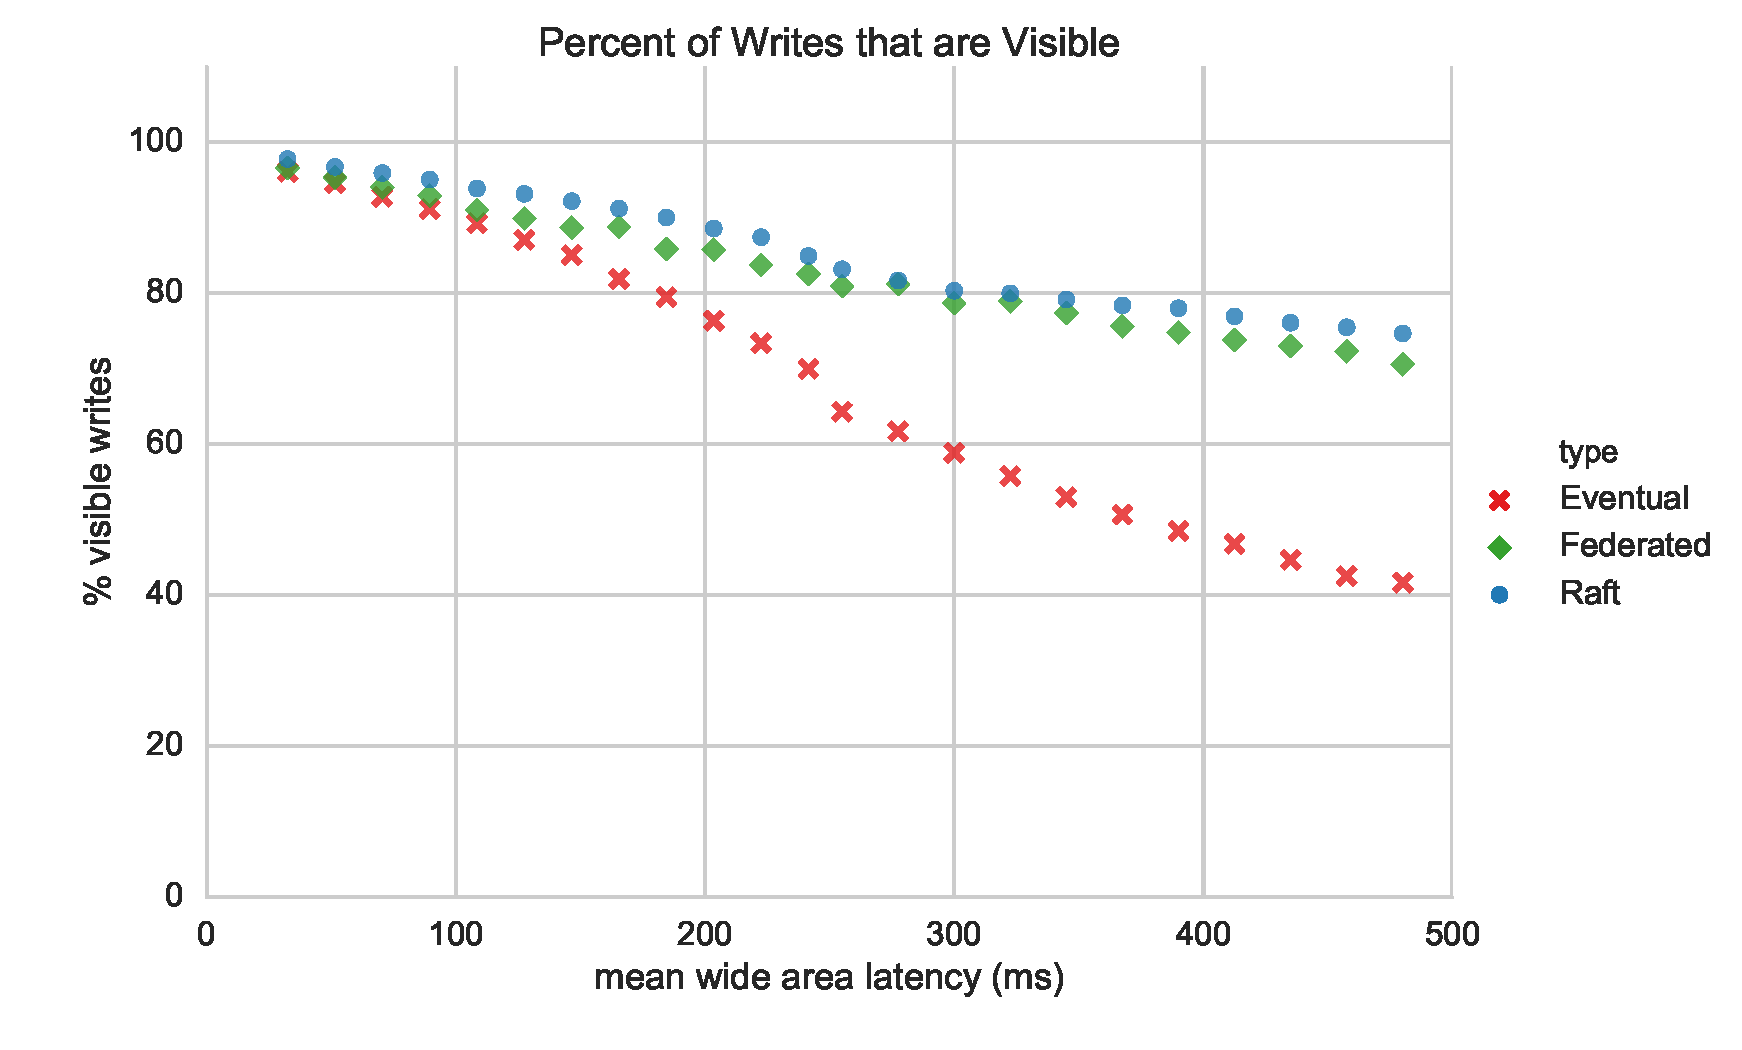
\includegraphics[width=\linewidth]{figures/latency/percent_visible_writes}
      \caption{The percentage of fully visible writes.}\label{fig:visible_writes}
    \endminipage\hfill
    \minipage{0.5\textwidth}%
      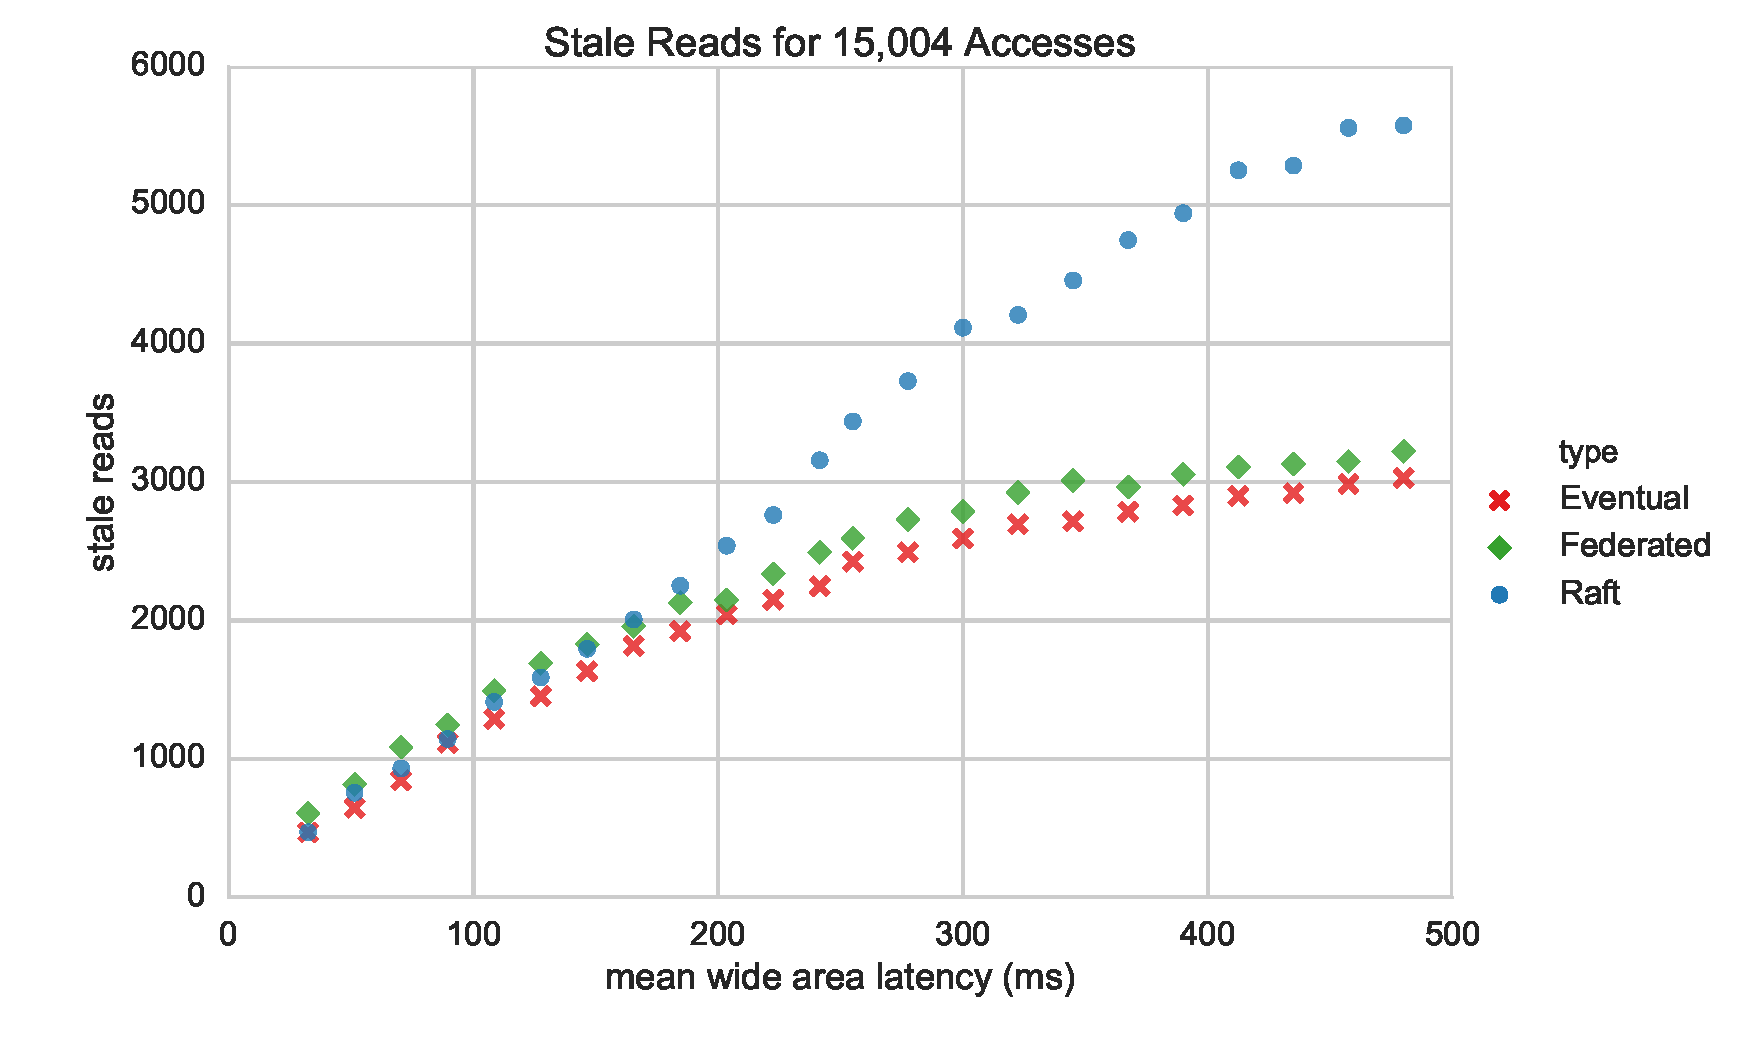
\includegraphics[width=\linewidth]{figures/latency/stale_reads}
      \caption{The percent of reads that are stale in the system.}\label{fig:latency_stale_reads}
    \endminipage
\end{figure*}

\subsection{Results}
\label{sec:results-1}

We investigate the effect of variable latency and the network environment on consistency
by constructing a fully connected topology of replicas distributed among several
geographic regions.
Within each region, replicas enjoy stable, low-latency connections with their neighbors.
The latency is higher and the connections more variable across regions, meaning that out
of order messages are more common across the wide area than in the local area.
We built a discrete event network simulation that allows us to flexibly configure network
and workload parameters.
Our eventual replicas replicate via anti-entropy with random neighbors selected for
gossip.
Raft nodes implement the Raft consensus protocol, using the replicated log to build a
total ordering on committed writes.

\subsection{Experiments and Metrics}

In this paper we concentrate on two of our latency variation results.
Each simulation is parameterized by a $T$ parameter that is a function of the
wide area mean ($\lambda_{\mu}$) and standard deviation ($\lambda_{\sigma}$).
However, the access mean, $A_{\mu}$ was fixed at approximately one access per replica every
3000ms.
In effect, this meant that for approximately half the simulations (with the higher
latencies), it was impossible for a write to become visible on another replica before a
fork.
Figure~\ref{fig:visible_writes} shows that
write propagation is much faster and more effective in Raft than in Eventual,
especially as network conditions deteriorate, and 
closely tracks the number of writes fully
replicated by Raft.

The strong inner core of Raft replicas is the key to the Federated protocol
tracking Raft's performance.
Eventual replicas are biased in favor of performing anti-entropy with local
replicas, allowing most anti-entropy sessions to perform quickly and without
delay.
By contrast, the Raft replicas in our Federated topology are intentionally
spread across geographic regions.
A new write originating at an Eventual replica is quickly spread to the local
Raft replica, and is then broadcast to the rest of the regions via the Raft
\texttt{AppendEntries} message.
Disseminating writes quickly minimizes the possibility of another, later
Eventual write starting up concurrently.
Additionally, the Forte number prevents new forked writes from stomping on a
conflicting write disseminated via Raft replicas.

Figure~\ref{fig:latency_stale_reads} shows
the average number of stale reads and forked writes across different mean
latencies.
All three protocols perform similarly at smaller latencies, but Eventual and
Federated deal with high latencies much more effectively than Raft, at least
for this size of system.

Higher latencies affect Raft in at least two ways.
First, higher latency variability causes more out of order messages.
Second, we parameterize system timeouts by $T$ which, in turn, is based on
mean latencies.
The result is that Raft's \texttt{AppendEntries} delay is longer for
simulations with higher mean latencies, resulting in more conflicts.
The same is true for anti-entropy delays, but the speed of Raft decisions is
determined by the slowest quorum member, which can be quite slow when message
variability is large.
By contrast, a slow anti-entropy participant only affects direct anti-entropy
partners.

\vspace{.5em}
\section{Discussion \& Conclusion}
\label{sec:conclusion}

This paper has presented a model for Federated consistency, which allows individual
replicas to expose local policies to users, while still allowing for global guarantees.
We evaluate Federated consistency in the context of a geographically dispersed wide-area
file system.
Our results show that a key to the global guarantees is in using a core
strongly-consistent group to serialize and broadcast system writes.
By designing a Federated system where only the interactions between replicas of varying
consistency types are defined, systems can scale beyond the handful of devices usually
described to dozens or hundreds of replicas in variable-latency, partition-prone
geographic networks.
Replicas can monitor their local environment and adapt as necessary to meet timeliness and
correctness constraints required by the local user.

% \section*{Acknowledgments}
%
% Thank you Bluejacket, for tirelessly running simulations as soon as we spun you up.

\bibliographystyle{plain}
\bibliography{references}


\end{document}
